\documentclass[a4paper,12pt]{report}
\usepackage[utf8]{inputenc}
\usepackage{lmodern}
\usepackage{enumitem}
\usepackage{titlesec}
\usepackage{graphicx}
\usepackage{tabularx}
\usepackage{amsmath}
\usepackage{amssymb}
\usepackage{verbatim}
\usepackage[italian]{babel}
\usepackage[margin=2cm]{geometry}
\usepackage{newunicodechar}

\newunicodechar{≠}{\ensuremath{\neq}}

\title{Progetto 20080110 - (P.20080110) - QuickHospital}
\author{Sebastiano Deodati}

\titleformat{\chapter}[display]{\normalfont\huge\bfseries}{}{0pt}{\Huge}

\begin{document}
  \maketitle
  \tableofcontents

  \chapter{Dati di interesse e funzionalità richieste}
    \begin{enumerate}[label*=\arabic*.]
        \item Personale
        \begin{enumerate}[label*=\arabic*.]
            \item Nome
            \item Cognome
            \item Data di nascita
            \item Pazienti
            \begin{enumerate}[label*=\arabic*.]
                \item Telefono
                \item Email
                \item Casella postale
                \item Pazienti esterni
                \begin{enumerate}[label*=\arabic*.]
                    \item Medico curante (req. 1.5)
                    \item Prestazione richiesta (req. 5)
                \end{enumerate}
            \end{enumerate}
        \end{enumerate}
        \item Medici
        \begin{enumerate}[label*=\arabic*.]
            \item Specializzazione primaria (req. 6)
            \item Eventuali specializzazioni secondarie (req. 6)
            \item Pazienti (req. 1.4)
        \end{enumerate}
        \item Stanze
        \begin{enumerate}[label*=\arabic*.]
            \item Piano
            \item Settore
            \item Posti letto (da 1 a 8) (req. 3)
        \end{enumerate}
        \item Posti letto
        \begin{enumerate}[label*=\arabic*.]
            \item Disponibilità
        \end{enumerate}
        \item Ricoveri
        \begin{enumerate}[label*=\arabic*.]
            \item Paziente (req. 1.4)
            \item Posto letto (req. 3)
        \end{enumerate}
        \item Prestazione medica
        \begin{enumerate}[label*=\arabic*.]
            \item Specializzazione (req. 6)
            \item Descrizione
        \end{enumerate}
        \item Specializzazione
        \begin{enumerate}[label*=\arabic*.]
            \item Nome
        \end{enumerate}
        \item Funzionalità richieste:
        \begin{enumerate}[label*=\arabic*.]
            \item Il sistema deve consentire al personale di accettazione di registrare ricoveri e dimissioni dei pazienti
            \item Il sistema deve assistere i medici nel programmare il loro itinerario di visite, cioè un insieme ordinato di stanze da visitare, dato da tutte e sole le stanze in cui sono ricoverati pazienti in cura presso quel medico. L'itinerario deve essere ottimizzato tramite ordinamento in primo luogo rispetto al piano, e in secondo luogo rispetto al settore
            \item Il sistema deve consentire, data una prestazione esterna di specializzazione \textit{s} richiesta da un paziente esterno, di ottenere l'insieme dei medici maggiormente idonei ad erogarla. In particolare, se esistono medici con specializzazione primaria \textit{s}, viene restituito l'insieme di tali medici, altrimenti viene restituito l'insieme dei medici che hanno \textit{s} tra le specializzazioni secondarie
        \end{enumerate}
    \end{enumerate}

    \chapter{Diagramma ER}
      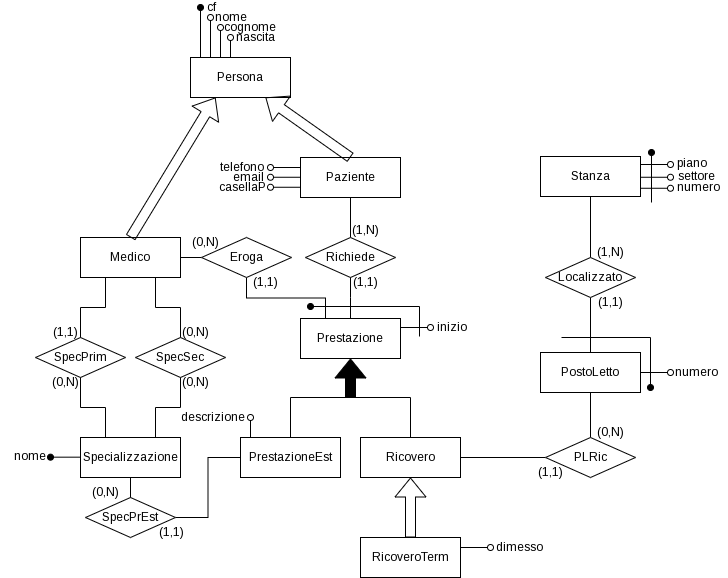
\includegraphics[width=1\textwidth]{er.png}
    \chapter{Dizionario dei dati}
      \section*{Entità Persona}
        \begin{tabular}{|c|c|c|}
	        \hline attributo & tipo & note \\
	        \hline cf & cf\_t & introdotto per identiticare univocamente le persone \\
	        \hline nome & stringa & \\
	        \hline cognome & stringa & \\
	        \hline nascita & data & \\
	        \hline
        \end{tabular} \\

      \section*{Entità Paziente}
        \begin{tabular}{|c|c|c|}
	        \hline attributo & tipo & note \\
	        \hline telefono & numtel & \\
	        \hline email & email\_t & \\
	        \hline casellaP & indirizzo & \\
	        \hline
        \end{tabular} \\
        V.Paziente.ricoveri: $\forall p,r,i \, $Paziente$(p) \,\wedge\, $Ricovero$(r) \,\wedge\, $Richiede$(p, r) \\
        \hspace*{1cm}\wedge\, $inizio$(r, i) \,\wedge\, \neg\exists d\, [$dimesso$(r, d)] \;\rightarrow\; \neg\exists i' > i,r' \neq r \, [$Richiede$(p, r') \,\wedge\, $inizio$(r', i')]$ \\
        (finché il paziente non è dimesso, non può essere ricoverato né richiedere prestazioni sanitarie) \\

      \section*{Entità PostoLetto}
        \begin{tabular}{|c|c|c|}
	        \hline attributo & tipo & note \\
	        \hline numero & intero[1,8] & \\
	        \hline
        \end{tabular} \\

      \section*{Entità Stanza}
        \begin{tabular}{|c|c|c|}
	        \hline attributo & tipo & note \\
	        \hline piano & intero & 0 indica piano terra, numeri negativi indicano sotterranei \\
	        \hline settore & intero $>$ 0 & \\
	        \hline numero & intero $>$ 0 & \\
	        \hline
        \end{tabular} \\

      \section*{Entità Specializzazione}
        \begin{tabular}{|c|c|c|}
	        \hline attributo & tipo & note \\
	        \hline nome & stringa & \\
	        \hline
        \end{tabular} \\

      \section*{Entità Prestazione}
        \begin{tabular}{|c|c|c|}
	        \hline attributo & tipo & note \\
	        \hline inizio & dataora & \\
	        \hline
        \end{tabular} \\

      \section*{Entità PrestazioneEst}
        \begin{tabular}{|c|c|c|}
	        \hline attributo & tipo & note \\
	        \hline descrizione & stringa & \\
	        \hline
        \end{tabular} \\

      \section*{Entità RicoveroTerm}
        \begin{tabular}{|c|c|c|}
	        \hline attributo & tipo & note \\
	        \hline dimesso & dataora & \\
	        \hline
        \end{tabular} \\
        V.RicoveroTerm.dimissione: $\forall r,i,f\;\;$Ricovero$(r) \;\wedge\; $inizio$(r, i) \;\wedge\; $dimesso$(r, f) \\
        \hspace*{1cm}\rightarrow i \;\leq\; f$ \\

      \section{Tipi di dati personalizzati}
        cf\_t: stringa in formato codice fiscale \\
        numtel: stringa che rappresenta un numero di telefono valido \\
        email\_t: stringa che rappresenta un'email valida \\
        indirizzo: record:
        \begin{itemize}
          \item via\_pza: stringa
          \item civico: intero $\leq$ 0 (0 per SNC)
          \item CAP: stringa CAP (5 cifre)
          \item Città: stringa
        \end{itemize}

    \chapter{UML}
      \begin{center}
        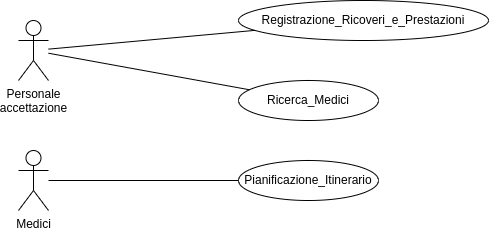
\includegraphics{uml.png}
      \end{center}

    \chapter{Specifiche degli use-case}
      \section{Specifiche use-case Registrazione\_Ricoveri\_e\_Prestazioni}
        \hspace*{1cm}Registra\_Paziente(cf: cf\_t, nome: stringa, cognome: stringa, nascita: data, \\
        \hspace*{3cm}telefono: numtel, email: email\_t, casella: indirizzo) : Paziente \\
        \hspace*{2cm}precondizioni: $\neg \exists p [\text{Paziente}(p) \wedge \text{cf}(p, cf)] \wedge \text{nascita} \leq \textit{oggi}$ \\
        \hspace*{2cm}postcondizioni: \\
        \hspace*{3cm}modifica al livello estensionale dei dati: \\
        \hspace*{4cm}nuovi elementi del dominio di interpretazione: p \\
        \hspace*{4cm}nuove ennuple di predicati: \\
        \hspace*{5cm}Persona(p) \\
        \hspace*{5cm}Paziente(p) \\
        \hspace*{5cm}cf(p, cf) \\
        \hspace*{5cm}nome(p, nome) \\
        \hspace*{5cm}cognome(p, cognome) \\
        \hspace*{5cm}nascita(p, nascita) \\
        \hspace*{5cm}telefono(p, telefono) \\
        \hspace*{5cm}email(p, email) \\
        \hspace*{5cm}casellaP(p, casella) \\
        \hspace*{3cm}valore di ritorno: result = p \\

        \hspace*{-0.75cm}
        \hspace*{1cm}Registra\_Ricovero(p: Paziente, medico: Medico, pl: PostoLetto) : Ricovero \\
        \hspace*{2cm}precondizioni: $\forall r \text{ Ricovero}(r) \wedge \text{Richiede}(p, r) \exists d [\text{dimesso}(r, d)]$ \\
        \hspace*{2cm}postcondizioni: \\
        \hspace*{3cm}modifica al livello estensionale dei dati: \\
        \hspace*{4cm}nuovi elementi del dominio di interpretazione: r \\
        \hspace*{4cm}nuove ennuple di predicati: \\
        \hspace*{5cm}Ricovero(r) \\
        \hspace*{5cm}Richiede(p, r) \\
        \hspace*{5cm}Eroga(medico, r) \\
        \hspace*{5cm}inizio(r, \textit{adesso}) \\
        \hspace*{3cm}valore di ritorno: result = r \\

        \newpage

        \hspace*{-0.75cm}
        \hspace*{1cm}Dimetti(r: Ricovero) : RicoveroTerm \\
        \hspace*{2cm}precondizioni: nessuna \\
        \hspace*{2cm}postcondizioni: \\
        \hspace*{3cm}modifica al livello estensionale dei dati: \\
        \hspace*{4cm}dominio di interpretazione: invariato \\
        \hspace*{4cm}nuove ennuple di predicati: \\
        \hspace*{5cm}RicoveroTerm(r) \\
        \hspace*{5cm}dimesso(r, \textit{adesso}) \\
        \hspace*{3cm}valore di ritorno: result = r \\

        \hspace*{-0.75cm}
        \hspace*{1cm}Registra\_Prestazione(p: Paziente, medico: Medico, desc: Descrizione, \\
        \hspace*{3cm}spec: Specializzazione) : PrestazioneEst \\
        \hspace*{2cm}precondizioni: $\text{SpecPrim}(medico, spec) \vee \text{SpecSec}(medico, spec)$ \\
        \hspace*{2cm}postcondizioni: \\
        \hspace*{3cm}modifica al livello estensionale dei dati: \\
        \hspace*{4cm}nuovi elementi del dominio di interpretazione: pr \\
        \hspace*{4cm}nuove ennuple di predicati: \\
        \hspace*{5cm}PrestazioneEst(pr) \\
        \hspace*{5cm}Richiede(p, pr) \\
        \hspace*{5cm}Eroga(medico, pr) \\
        \hspace*{5cm}SpecPrEst(pr, spec) \\
        \hspace*{5cm}inizio(pr, \textit{adesso}) \\
        \hspace*{5cm}descrizione(pr, desc) \\
        \hspace*{3cm}valore di ritorno: result = pr \\

      \section{Specifiche use-case Ricerca\_Medici}
        \hspace*{1cm}Ricerca\_Medico(spec: Specializzazione) : Medico(0,N) \\
        \hspace*{2cm}precondizioni: nessuna \\
        \hspace*{2cm}postcondizioni: \\
        \hspace*{3cm}modifica al livello estensionale dei dati: nessuna \\
        \hspace*{3cm}valore di ritorno: \\
        \hspace*{4cm}sia $S_1 = \{m | \text{Medico}(m) \wedge \text{SpecPrim}(m, spec)\}$ \\
        \hspace*{4cm}sia $S_2 = \{m | \text{Medico}(m) \wedge \text{SpecSec}(m, spec)\}$ \\
        \hspace*{4cm}result = $S_1$ se $|S_1| > 0$ $S_2$ altrimenti \\

      \newpage

      \section{Specifiche use-case Pianificazione\_Itinerario}
        \hspace*{1cm}Pianifica\_Itinerario(m: Medico) : (intero, intero)(0,N) \\
        \hspace*{2cm}precondizioni: nessuna \\
        \hspace*{2cm}postcondizioni: \\
        \hspace*{3cm}modifica al livello estensionale dei dati: nessuna \\
        \hspace*{3cm}valore di ritorno: \\
        \hspace*{4cm}sia $P = \{(r, pa, pl, s, p, st) | \text{Ricovero}(r) \wedge \text{Richiede}(pa, r) \wedge \text{Eroga}(m, r) \\
        \hspace*{5cm}\wedge \text{PLRic}(r, pl) \wedge \text{Localizzato}(pl, s) \wedge \text{piano}(s, p) \wedge \text{settore}(s, st)\}$ \\
        \hspace*{4cm}sia $it = \{(p, st) \forall (r, pa, pl, s, p, st) \in P\}$ \\
        \hspace*{4cm}result = $it$ ordinato per $p$ in primo luogo, per $st$ in secondo luogo \\

    \chapter{Scelta del DBMS}
      Il database verrà implementato sul DBMS PostGreSQL.

    \chapter{Ristrutturazione del diagramma ER}
      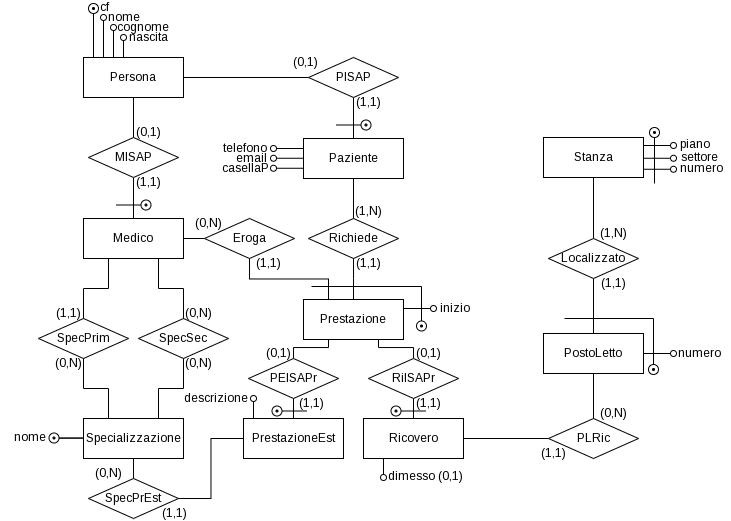
\includegraphics[width=1\textwidth]{er_ristr.png}
    \chapter{Transizione dei tipi di dati concettuali in tipi standard SQL}
      \section*{Entità Persona}
        \begin{tabular}{|c|c|c|}
	        \hline attributo & tipo & note \\
	        \hline cf & cf\_t & introdotto per identiticare univocamente le persone \\
	        \hline nome & stringM & \\
	        \hline cognome & stringM & \\
	        \hline nascita & date & \\
	        \hline
        \end{tabular} \\

      \section*{Entità Paziente}
        \begin{tabular}{|c|c|c|}
	        \hline attributo & tipo & note \\
	        \hline telefono & numtel & \\
	        \hline email & email\_t & \\
	        \hline casellaP & indirizzo & \\
	        \hline
        \end{tabular} \\
        V.Paziente.isa: $\forall pa \, $Paziente$(p) \;\rightarrow\; \exists p \, $PISAP$(pa, p)$ \\
        V.Paziente.ricoveri: $\forall p,r,pr,i \, $Paziente$(p) \,\wedge\, $Richiede$(p, pr) \,\wedge\, $RiISAPr$(r, pr) \\
        \hspace*{1cm}\wedge\, $inizio$(pr, i) \,\wedge\, \neg\exists d\, [$dimesso$(r, d)] \\
        \hspace*{1cm}\rightarrow\; \neg\exists i' > i,pr' \neq r \, [$Richiede$(p, pr') \,\wedge\, $inizio$(pr', i')]$ \\
        (finché il paziente non è dimesso, non può essere ricoverato né richiedere prestazioni sanitarie) \\

      \section*{Entità Medico}
        V.Medico.isa: $\forall m \, $Medico$(m) \;\rightarrow\; \exists p \, $MISAP$(m, p)$ \\

      \section*{Entità PostoLetto}
        \begin{tabular}{|c|c|c|}
	        \hline attributo & tipo & note \\
	        \hline numero & pl\_t & \\
	        \hline
        \end{tabular} \\

      \section*{Entità Stanza}
        \begin{tabular}{|c|c|c|}
	        \hline attributo & tipo & note \\
	        \hline piano & integer & 0 indica piano terra, numeri negativi indicano sotterranei \\
	        \hline settore & int\_pos & \\
	        \hline numero & int\_pos & \\
	        \hline
        \end{tabular}

      \section*{Entità Specializzazione}
        \begin{tabular}{|c|c|c|}
	        \hline attributo & tipo & note \\
	        \hline nome & stringL & \\
	        \hline
        \end{tabular}

      \section*{Entità Prestazione}
        \begin{tabular}{|c|c|c|}
	        \hline attributo & tipo & note \\
	        \hline inizio & datetime & \\
	        \hline
        \end{tabular} \\
        V.Prestazione.isa: $\forall p \, $Prestazione$(p) \;\rightarrow\; [\exists pr $RiISAPr$(pr, p)] \vee [\exists pe $PEISAPr$(pe, p)]$ \\
        V.Prestazione.disg: $\forall p \, $Prestazione$(p) \;\rightarrow\; [\exists pr $RiISAPr$(pr, p)] \;\rightarrow\; [\neg\exists pe $PEISAPr$(pe, p)]$

      \section*{Entità PrestazioneEst}
        \begin{tabular}{|c|c|c|}
	        \hline attributo & tipo & note \\
	        \hline descrizione & stringL & \\
	        \hline
        \end{tabular}

      \section*{Entità Ricovero}
        \begin{tabular}{|c|c|c|}
	        \hline attributo & tipo & note \\
	        \hline dimesso(0,1) & datetime & NULL indica che il paziente non è ancora stato dimesso \\
	        \hline
        \end{tabular} \\
        V.Ricovero.dimissione: $\forall p,r,i,f\;\;$Prestazione$(p) \;\wedge\; $inizio$(r, i) \;\wedge\; $RiISAPr$(r, p) \;\wedge\; $dimesso$(r, f) \\
        \hspace*{1cm}\rightarrow i \;\leq\; f$

      \newpage

      \section{Tipi di dati personalizzati}
        \texttt{create domain stringM as varchar(50)}; \\
        \texttt{create domain stringL as varchar(100)}; \\
        \texttt{create domain int\_pos as integer check value $>$ 0;} \\
        \texttt{create domain pl\_t as integer check value between 1 and 8;} \\
        \texttt{create domain cf\_t as char(16) \\
        \hspace*{1cm}check value \textasciitilde * '\textasciicircum[a-z]\{6\}[0-9]\{2\}[a-z][0-9]\{2\}[a-z][0-9]\{3\}[a-z]\$';} \\
        \texttt{create domain numtel as char(13) check value \textasciitilde * '\textasciicircum\textbackslash+[0-9]\{12\}\$';} \\
        \texttt{create domain email\_t as stringL check value \textasciitilde * '\textasciicircum[a-z0-9\_.-]+@[a-z0-9\_.-]+\textbackslash.[a-z]+\$';} \\
        \texttt{create type indirizzo ( \\
        \hspace*{1cm}via\_pza stringL not null, \\
        \hspace*{1cm}civico int\_pos, \hspace*{1cm} // NULL per SNC \\
        \hspace*{1cm}cap char(5) not null check value \textasciitilde * '\textasciicircum[0-9]\{5\}\$', \\
        \hspace*{1cm}citta stringM not null \\
        );} \\

    \chapter{Schema concettuale}
      Persona(\underline{cf}: cf\_t, nome: stringM, cognome: stringM, nascita: date) \\
      \hspace*{1cm}vincolo ennupla: nascita $\leq$ CURRENT\_DATE \\

      \hspace*{-0.75cm}
      Paziente(\underline{cf}: cf\_t, telefono: numtel, email: email\_t, casellaP: indirizzo) \\
      \hspace*{1cm}vincolo foreign key: (cf) references Persona(cf) \\
      \hspace*{1cm}vincolo ennupla: (cf) $\subseteq$ Prestazione(paziente) \\

      \hspace*{-0.75cm}
      Medico(\underline{cf}: cf\_t, specPrim: stringL) \\
      \hspace*{1cm}vincolo foreign key: (cf) references Persona(cf) \\
      \hspace*{1cm}vincolo foreign key: (specPrim) references Specializzazione(nome) \\

      \hspace*{-0.75cm}
      SpecSec(\underline{medico}: cf\_t, \underline{spec}: stringL) \\
      \hspace*{1cm}vincolo foreign key: (cf) references Medico(cf) \\
      \hspace*{1cm}vincolo foreign key: (spec) references Specializzazione(nome) \\

      \hspace*{-0.75cm}
      PostoLetto(\underline{numero}: pl\_t, \underline{piano}: integer, \underline{settore}: int\_pos, \underline{stanza}: int\_pos) \\
      \hspace*{1cm} vincolo foreign key: (piano, settore, stanza) references Stanza(piano, settore, numero) \\

      \hspace*{-0.75cm}
      Stanza(\underline{numero}: int\_pos, \underline{piano}: integer, \underline{settore}: int\_pos) \\

      \hspace*{-0.75cm}
      Specializzazione(\underline{nome}: stringL) \\

      \hspace*{-0.75cm}
      Prestazione(\underline{paziente}: cf\_t, \underline{medico}: cf\_t, \underline{inizio}: datetime) \\
      \hspace*{1cm}vincolo foreign key: (paziente) references Paziente(cf) \\
      \hspace*{1cm}vincolo foreign key: (medico) references Medico(cf) \\

      \hspace*{-0.75cm}
      PrestazioneEst(\underline{paziente}: cf\_t, \underline{medico}: cf\_t, \underline{inizio}: datetime, specializzazione: stringL, descrizione: stringL) \\
      \hspace*{1cm}vincolo foreign key: (paziente, medico) references Prestazione(paziente, medico) \\
      \hspace*{1cm}vincolo foreign key: (specializzazione) references Specializzazione(nome) \\

      \hspace*{-0.75cm}
      Ricovero(\underline{paziente}: cf\_t, \underline{medico}: cf\_t, \underline{inizio}: datetime, dimesso*: datetime, \\
      \hspace*{2cm}npl: pl\_t, ppl: integer, spl: int\_pos, stpl: int\_pos) \\
      \hspace*{1cm}vincolo foreign key: (paziente, medico) references Prestazione(paziente, medico) \\
      \hspace*{1cm}vincolo foreign key: (npl, ppl, spl, stpl) references \\
      \hspace*{2cm}PostoLetto(numero, piano, settore, stanza) \\
      \hspace*{1cm}vincolo ennupla: (inizio $\leq$ dimesso) or (dimesso = NULL) \\

    \chapter{Progettazione dei vincoli esterni}
      \begin{tiny}
        \verbatiminput{trigger.txt}
      \end{tiny}

    \chapter{Specifiche realizzative degli use-case}
      \begin{tiny}
        \verbatiminput{use-case.txt}
      \end{tiny}
    
\end{document}
